\documentclass[letterpaper,10pt]{article}
\usepackage[utf8]{inputenc}
\usepackage{hyperref}
\hypersetup{
    colorlinks=true,
    linkcolor=black,
    filecolor=magenta,      
    urlcolor=blue,
    citecolor=cyan,
    pdftitle={Overleaf Example},
    pdfpagemode=FullScreen,
    }
\usepackage{graphicx}
\graphicspath{ {images/} }
\usepackage[
backend=biber,
style=alphabetic,
sorting=ynt
]{biblatex}
\addbibresource{project1_bibliography.bib}

\title{Projekt 1: \\ Klassifikation von Datteln mit einem neuronalem Netz in Keras}
\author{Philipp Petermeier \\
    \href{https://github.com/PPetermeier/SoSe2022_Machine_Learning}{Git-Archiv}
    }
\date{2022.06.05}

\begin{document}

\maketitle
\newpage
\renewcommand{\contentsname}{Inhaltsverzeichnis}
\tableofcontents
\newpage

\section{Überblick}
    Die Aufgabenstellung von Projekt 1 besteht darin, \href{https://www.kaggle.com/code/kaushikjegannathan/date-fruit-classification-using-ann}{diesen Datensatz} \cite{Koklu.2021}
    in dem Datteln anhand von numerischen Parametern kategorisiert werden zu nutzen, um mit Keras\cite{chollet2015keras} ein neuronales Netz zu bauen, mit dem die Klassen verlässlich vorhersagt werden können. Es sollen dabei geeignete Metriken und Tensorboard zur Darstellung genutzt werden, um das Modell zu optimieren. Folgende Schritten sollen im folgenden übersichtsartig dokumentiert werden:
    \begin{itemize}
        \item Exploration des Datensatzes mit Visualisierung
        \item Preprocessing
        \item Aufbau eines ersten Models
        \item Darstellung des Models mit Tensorboard
        \item Optimizierung mit KerasTuner
    \end{itemize}
    Das Git-Archiv ist frei verfügbar und organisiert um für das ganze Semester sinnvoll nutzbar zu sein: Jedes Projekt hat einen eigenen Ordner, mit Daten für die Aufgabenstellung, Code und Outputs. Von der main.py aus werden die einzelnen Projekte importiert und einfach aufgerufen, um einzelnes testen zu ermöglichen und die einzelnen hier besprochenen Schritte sind jeweils in einzelnen Methoden in project1.py abgespeichert. Der Ordner "PresentationCode"enthält die codebeispiele aus der Vorlesung, auf die zum Lernen teilweise zugegriffen wurde. Die Outputs umfassen mit python erstellte Grafiken, logs und modelle die zur Demonstration erstellt wurden, sowie die LaTeX-Dateien der Dokumentation selbst.


\newpage
\section{Datensatz}
    Als einen ersten Schritt gilt es den Datensatz nachzuvollziehen, zu diesem Zweck wurden die Funktionen von Pandas\cite{JeffReback.2020} 
    genutzt, da die Datei damit auch eingelesen und folgend auch bearbeitet wird. 
    \begin{figure}[h]
        \centering
        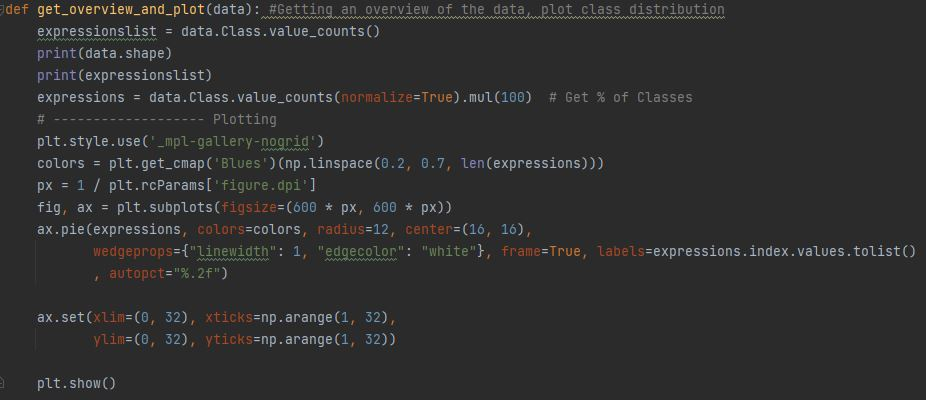
\includegraphics[width=\textwidth]{Output2.JPG}
        \caption{Pandas-Anweisungen für erste Übersicht}
        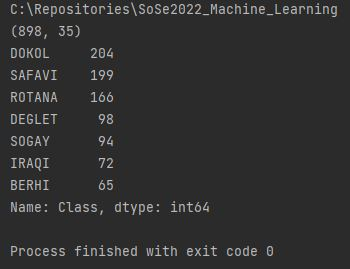
\includegraphics[width=0.5\textwidth]{Output1.JPG}
        \caption{Output des entsprechenden Codes}
    \end{figure}
    
    Wie zu sehen ist enthält der Datensatz 898 Einträge mit 35 Merkmalen, eines der Merkmale ist dabei die Zielklasse als String, welche es zu encoden gilt. Die anderen 34 sind floats, die lediglich normalisiert werden müssen. Ebenfalls zu sehen ist die Verteilung der einzelnen Klassen, deren ungleiche Verteilung bereits in der Aufgabenstellung angedeutet worden war. Es ist für ein sinnvolles Training also nötig, die Daten stratifiziert zu splitten um selection bias beim Training zu vermeiden.(siehe nächste Seite)
    \begin{figure} [p]
        \centering
        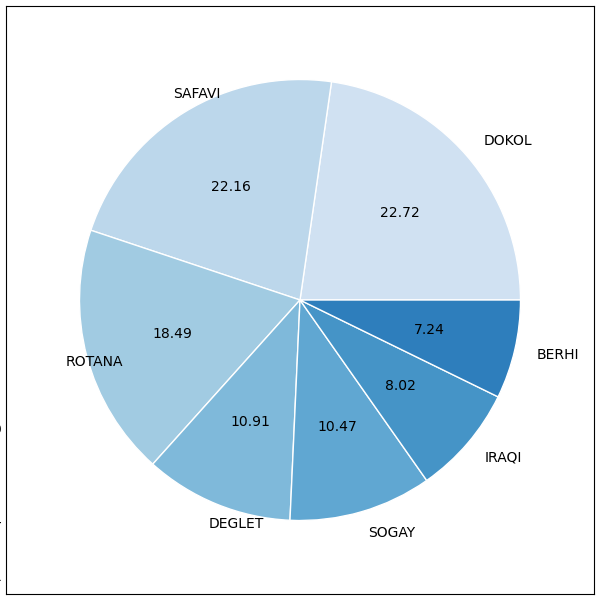
\includegraphics[width=\textwidth]{PieChart_ClassOverview.png}
        \caption{Prozentuale Verteilung der Klassen auf den Datensatz visualisiert in einem Kuchendiagramm, erstellt mit matplotlib \cite{Hunter.2007}}
    \end{figure}
        
\newpage
\section{Preprocessing}
    Das Preprocessing wurde nicht in einem Layer sondern einfach im Code erledigt. Die Zielklassen wurden einfach in einem Dictionary gespeichert, dann die Klassen-Spalte als ein neue Objekt definiert und mit to categorical von keras.util auf das dictionary gemapt. Der Datensatz wurde ebenfalls als neues Objekt gespeichert und dann mit dem standard-Scaler von Scikit \cite{Pedregosa.2011}
    normalisiert. Ebenfalls mit Scikit wurde der train-test-split getätigt. Es wurde ein 80-20 Split gewählt, ein random split festgelegt um die Ergebnisse reproduzierbar zu halten und vor allem die Stratifizierung der Daten auf True gesetzt, wie bereits im vorherigen Kapitel erwähnt.
    \begin{figure} [h]
        \centering
        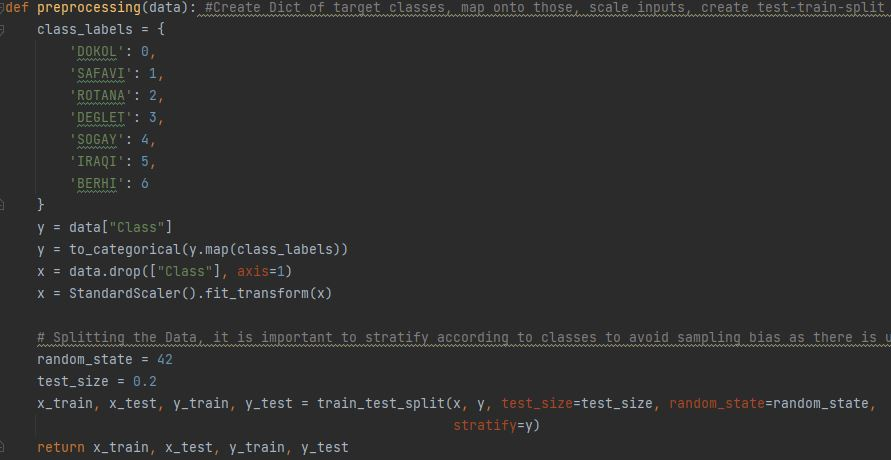
\includegraphics[width=\textwidth]{Preprocessing.JPG}
        \caption{Preprocessing-Code}
    \end{figure}

\newpage
\section{Modelbau}
    \begin{figure} [t]
        \centering
        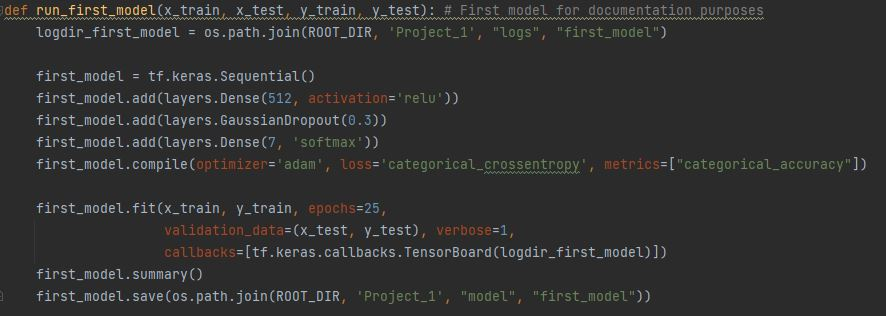
\includegraphics[width=\textwidth]{firstmodel.JPG}
        \caption{Konfiguration des ersten Models im Quellcode}
    \end{figure}
    Mit der Sequential-Klasse wird das model modular aufgebaut, es wurde lediglich ein breiter relu-aktivierter layer erstellt und ein gaussianDropout layer dahinter geschaltet um overfitting zu vermeiden. Im späteren Verlauf wurde der Dropout- durch einen Noise-Layer ersetzt. Die Aktivierungsfunktion für den Kategorie-Layer ist dann eine softmax, um die eingegangenen Information in Wahrscheinlichkeiten einer Klassenzugehörigkeit umzuwandeln. Die Verlustfunktion und Metriken wurden dem Klassifizierungsproblem mit mehr als 2 Klassen entsprechend gewählt. Das compilierte model wird danach in 25 Epochen trainiert, und das tracking auf einfachen Fortschrittsbar gesetzt, da der Trainingsverlauf mit der callbacks-Funktion an einem definiertem Ort gespeichert wird. Diese Daten werden folgend mit Tensorboard dargestellt, das model selbst wird kurz zusammengefasst und dann in einem eigenem Ordner gespeichert, sodass zu einem späterem Zeitpunkt erneut darauf zurück gegriffen werden kann.
    \begin{figure} [h]
        \centering
        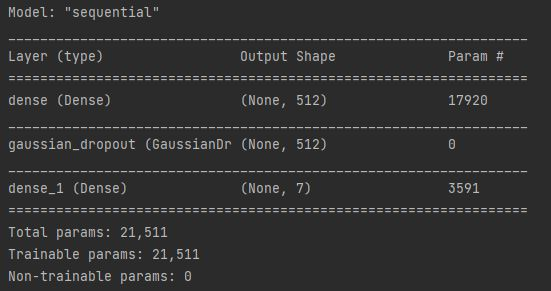
\includegraphics[width=0.75\textwidth]{firstmodel2.JPG}
        \caption{Zusammenfassung des erstellten models}
    \end{figure}
    
\newpage


\section{Tensorboard}
    \begin{figure} [t]
        \centering
        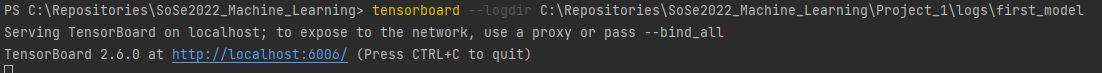
\includegraphics[width=\textwidth]{tensorboard_terminal.JPG}
        \caption{Start von Tensorboard im Terminal nach erfolgtem und geloggtem model-Training}
    \end{figure}
    Die Logs des Trainings des ersten models können nun mit Tensorboard ausgelesen werden. Tensorboard wird über das Terminal aufgerufen und benötigt den Ordnerpfad der Logs, die ausgewertet werden sollen. Diese Logs werden dann automatisiert aufbereitet, grafisch dargestellt und die Ergebnisse über einen Browser auf einem für Tensorboard freigegebenem lokalem Port zugänglich gemacht.
    \begin{figure} [h]
        \centering
        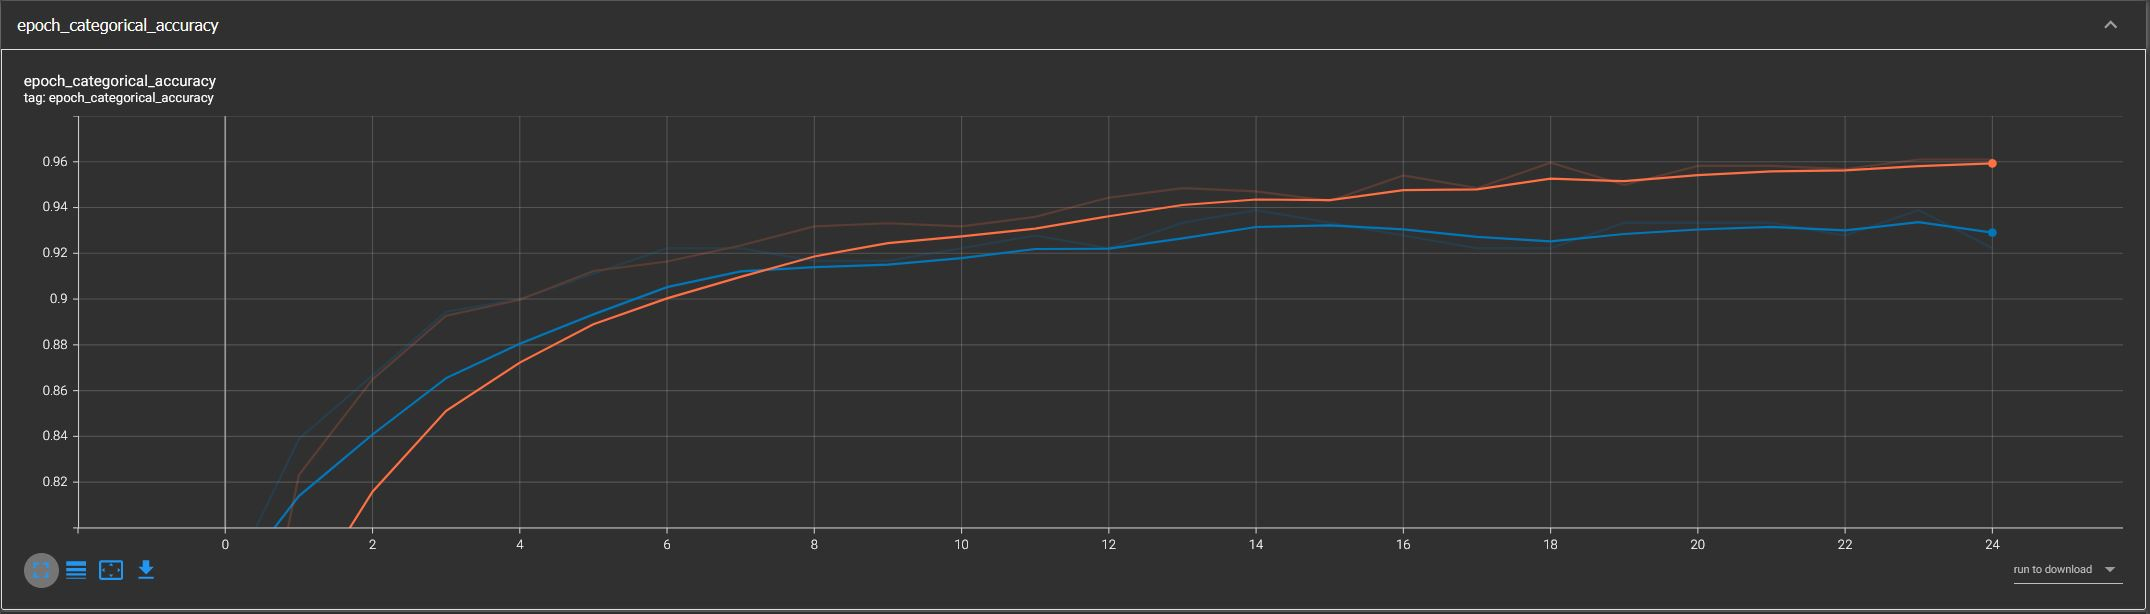
\includegraphics[width=\textwidth]{tensorboard_catAcc.JPG}
        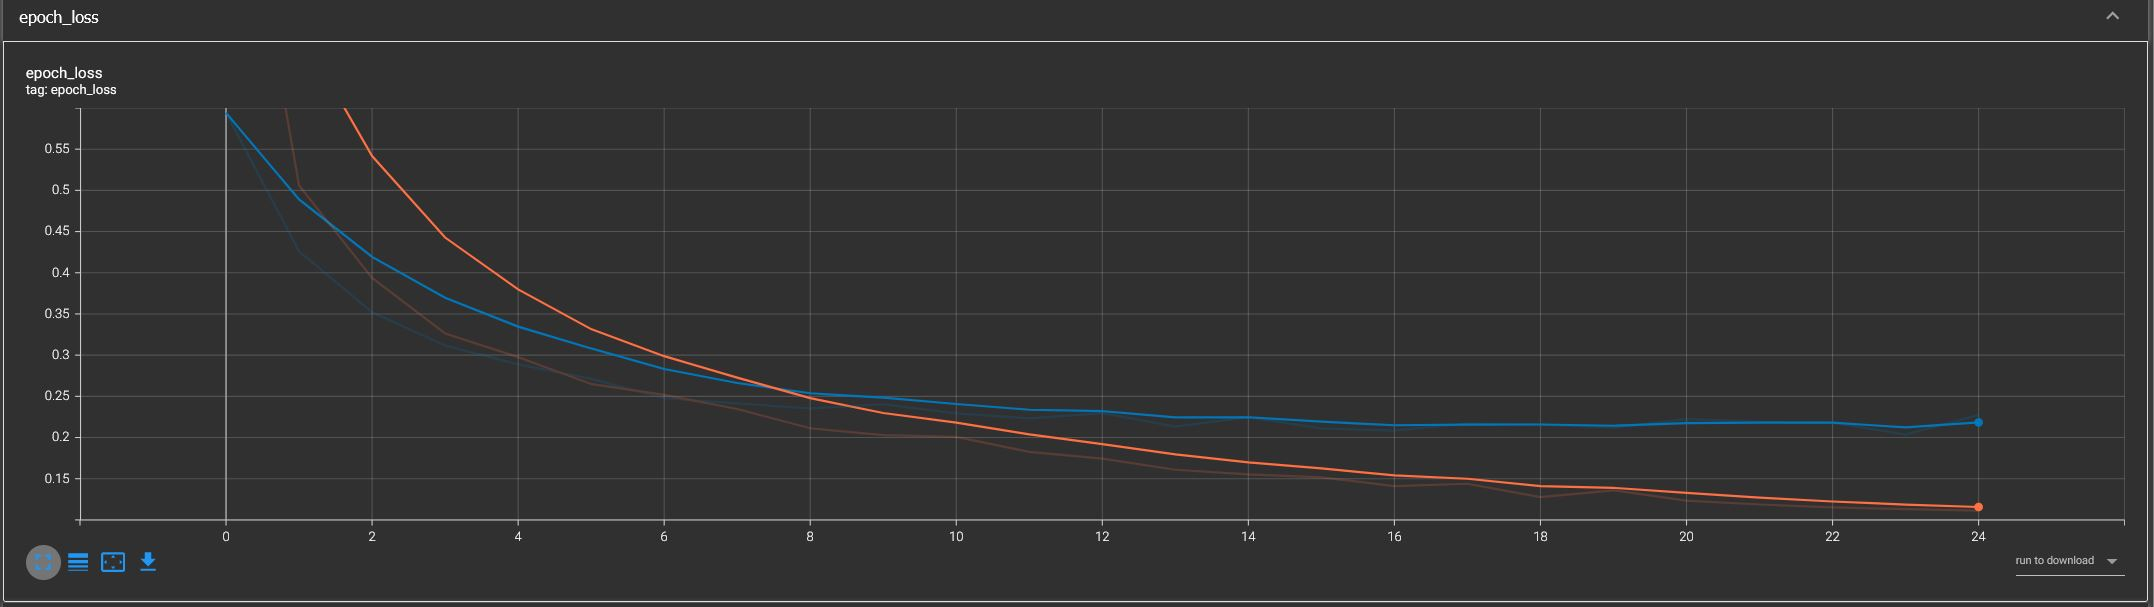
\includegraphics[width=\textwidth]{tensorboard_epocloss.JPG}       
        \caption{Von Tensorboard erstellte Plots der Trainingswerte: Kategoriale Genauigkeit und Epochenverlust}
    \end{figure}

\newpage

\section{KerasTuner}
    Mit dem KerasTuner\cite{OMalley.2019b} kann ein Keras-Model nach optimalen Hyperparametern untersucht werden. Die vom Tuner benötigten Inputs bestehen in einem Funktionsaufruf zum Aufbau eines Keras-Models mit flexiblen Parametern, welche den Suchraum definieren innerhalb dessen die Optimierung stattfindet. 
    Zunächst einmal muss in der buildModel-Methode entschieden werden, welche Hyperparameter überhaupt betrachtet werden sollen und welche fixiert sind. Gleichzeitig ist zumindest in diesem Fall auch zu beachten, dass die Anzahl der Layer, also die Architektur des Neuronalen Netzes fix gesetzt wird.
    \newline
    \begin{figure} [h!]
        \centering
        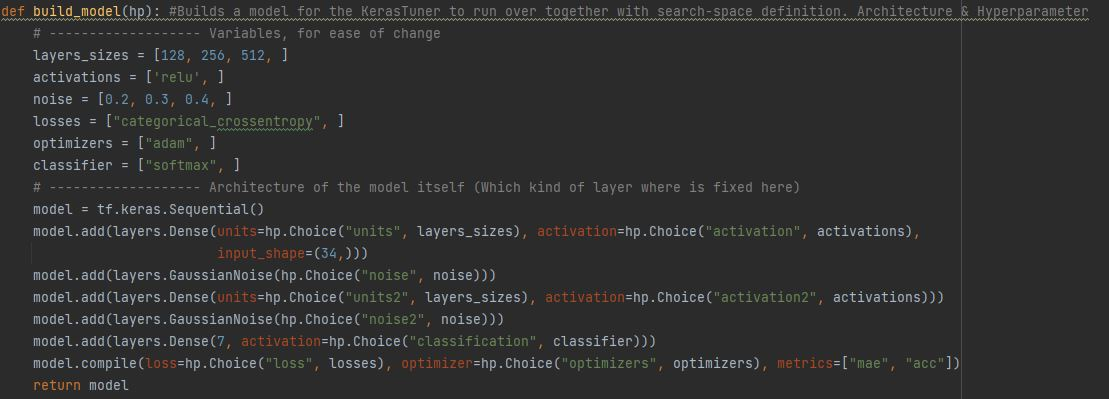
\includegraphics[width=\textwidth]{build_model.JPG}
        \caption{BuildModel Methode mit den vom KerasTuner gefundenen optimalen Parametern}
    \end{figure}
    \newpage
    Sobald die buildModel-Methode komplett ist, übergibt man dem KerasTuner diese, den Parameter auf den optimiert werden soll, weitere Anweisungen für die Anzahl und den Verlauf der Suche, wohin die Logs für Tensorboard, die den Verlauf der Suche dokumentieren, und wo das beste Modell gespeichert werden sollen, und ruft dann auf. Der KerasTuner läuft dann alle möglichen Konfigurationen durch (sofern diese nicht widersprüchlich sind weil beispielsweise geringere maximale Versuchsanzahl als Anzahl Konfigurationen), loggt und speichert hier im Repository das beste gefundene model. \\
     \begin{figure} [h!]
        \centering
        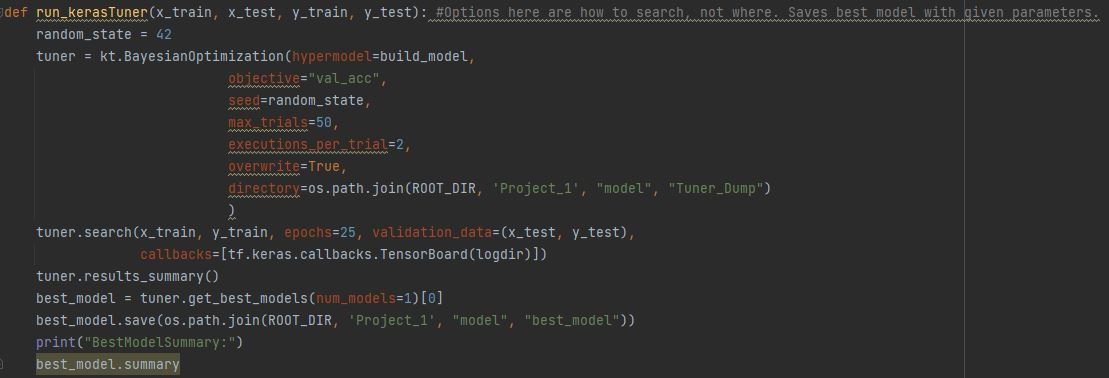
\includegraphics[width=\textwidth]{kerasTuner.JPG}
        \caption{KerasTuner-Methode mit den genutzten Konfigurationen}
    \end{figure}
    Die Konfigurationen von Verlustfunktion categorical crossentropy, Optimierer adam und Aktivierungsfunktion softmax für zu den Kategorienlayer hat sich definitiv als die beste herausgestellt, sodass hier keine Optionen mehr angegeben werden, um den Suchraum für einen Test klein zu halten. Die Werte für Layergröße und Noise-Konstanten sind in den Test so weit fluktuiert, dass die Änderungen wahrscheinlich im Toleranzbereich zu finden sind, weswegen die drei immer wieder gefundenen Werte jeweils aufgeführt sind. Sobald der Tuner einmal durchgelaufen ist kann man sich selbstverständlich den gesamten Verlauf des Tunings auf dem Tensorboard nachvollziehen um zu verstehen, welche Kombinationen wie sinnvoll sind, auch wenn der Tuner selbst sehr viel erledigt - er kann nur in dem Raum suchen, den er übergeben bekommt und hier ist die Intuition des Entwicklers entscheidend.
    Das hier beschriebene Vorgehen, zunächst das Problem präzise zu formulieren, die Daten gründlich zu betrachten und dann ein angemessenes erstes model zu entwerfen, um im späteren Verlauf mit dem KerasTuner zu testen, in welche Richtung Hyperparameter optimiert werden können hat sich als sehr sinnvoll dargestellt und wird bei den nächsten Aufgaben sicherlich ähnlich gehandhabt werden. 

\newpage

\section{Sicherung}
    Im Git-Archiv sind neben dem Code folgende Daten zu finden: Eine .yml mit allen benötigten Informationen um die virtuelle Umgebung mit conda problemlos aufsetzen zu können, Tensorboard-Logs des ersten models und des letzen Durchlaufes des KerasTuners unter /logs, sowie das erste und beste model, welche bei der aktuellen Konfiguration der Methoden einfach nur geladen und zusammengefasst geprintet werden. Der Verlauf des Trainings kann mit Tensorboard nachvollzogen werden, und sämtliche andere Funktionen können mit einem einfachen Aufruf von runproject1() in project1.py zu Test- oder Demonstationszwecken aufgerufen werden.

\newpage
\printbibliography

\end{document}
